%% -*- coding: utf-8 -*-
\documentclass[12pt,a4paper]{scrartcl} 
\usepackage[utf8]{inputenc}
\usepackage[english,russian]{babel}
\usepackage{indentfirst}
\usepackage{misccorr}
\usepackage{graphicx}
\usepackage{amsmath}
\usepackage{pgfplots}
\pgfplotsset{compat=1.9}
%Настройка стилей
\pgfplotsset{model/.style = {blue, samples = 100}}
\pgfplotsset{experiment/.style = {red}}


\begin{document}
\begin{titlepage}
  \begin{center}
    \large




    \vspace{0.5cm}

    Санкт-Петербургский политехнический университет Петра Великого
    \vspace{0.25cm}
    
    Институт компьютерных наук и технологий
    
    Программная инженерия
    \vfill
    
    
    Авферонок Александр Сергеевич
    \vfill

    \textsc{Лабораторная работа №4}\\[5mm]
    
    {\LARGE Определение опций оптимизации,\\
      для приложения}
  \bigskip
    
    1 курс, группа в13534/22
\end{center}
\vfill

\newlength{\ML}
\settowidth{\ML}{«\underline{\hspace{0.7cm}}» \underline{\hspace{2cm}}}
\hfill\begin{minipage}{0.4\textwidth}
  Преподователь\\
  \underline{\hspace{\ML}} А.\,В.~Петров\\
  «\underline{\hspace{0.7cm}}» \underline{\hspace{2cm}} 2019 г.
\end{minipage}%
\bigskip
\vfill

\begin{center}
  Санкт-Петербург, 2019 г.
\end{center}
\end{titlepage}
\newpage
Цель работы - написать сценарий, который будет компелировать программу с разными уровнями оптимизации, 
вычисление времени работы программы и вычисление занимаемого исполняемым файлом дискового пространства.
Сценарий должен принемать имя исходного файла.
\par
Исходный код компелируемого приложения:
\begin{verbatim}
    #include <stdio.h>
    
    double powern (double d, unsigned n) {
        double x = 1.0;
        unsigned j;
        for (j = 1; j <= n; j++)
	    x *= d;
        return x;
    }

    int main (void) {
        double sum = 0.0;
        unsigned i;
        for (i = 1; i <= 100000000; i++)
        {
	    sum += powern (i, i % 5);
        }
        printf ("sum = %g\n", sum);
        return 0;
    }
\end{verbatim}
Далее прдеставлена таблица и график для наглядного сравнения параметов исполняемого файла, сформированного по резултатом работы сценария.

\newpage
\begin{center}
\caption{Таблица 1: Результат компиляций приложения}
\begin{tabular}{| l | l | l |}
\hline
Ключ оптимизации & Время исполнения, сек & Размер, байт  \\ \hline
O0 & 762 & 8672\\
Os & 523 & 8672\\
O1 & 267 & 8672\\
O2 & 236 & 8672\\
O3 & 238 & 8672\\
O2 -march=native&	235&	8672\\
O3 -march=native &	236	&8672\\
O2 -march=native -funroll-loops&	240	&8672\\
O3 -march=native -funroll-loops&	245	&8672\\
O2 -march=native -flto&	236	&8608\\
O2 -march=native -fipa-reference&	234	&8672\\
O2 -march=native -fprofile-generate& 569	&28920\\
O2 -march=native -fprofile-use&	169	&8672\\
O2 -march=native -flto -fprofile-use&	163	&8608\\
O2 -march=native -fipa-reference -fprofile-use&	168	&8672\\
O2 -march=native -flto -fprofile-generate	&585	&28888\\
O2 -march=native -fipa-reference -fprofile-generate & 563 &	28920\\
\hline
\end{tabular}\\

\parindent=1cm
\caption{Рисунок 1.}
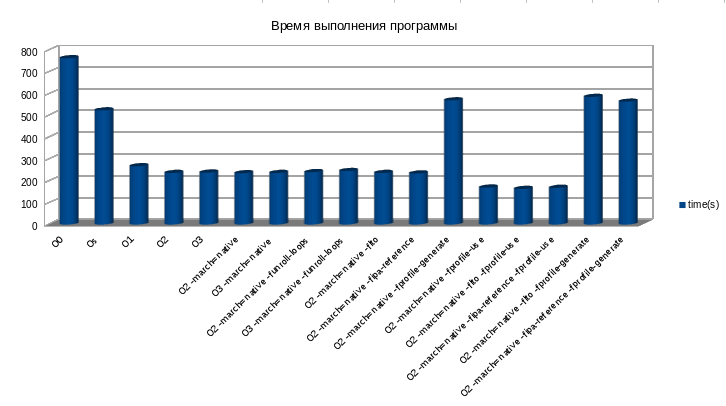
\includegraphics[width=\linewidth]{time.PNG}
\newpage
\caption{Рисунок 2.}
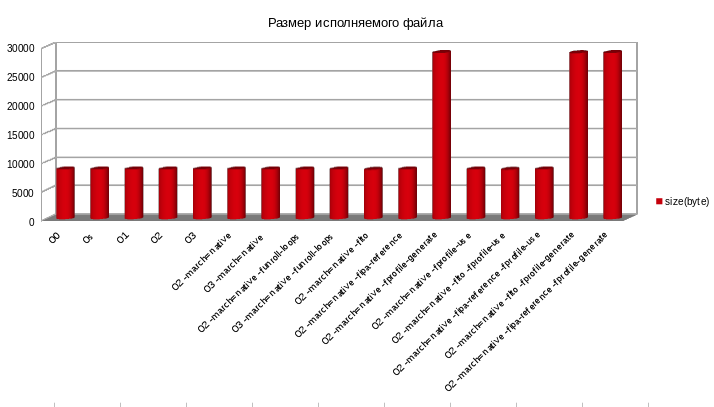
\includegraphics[width=\linewidth]{size.PNG}
\end{center}
\par
Вывод, в результате выполнения лабораторной работы было выявленно, 
что размер файла не изменялся до использования межпроцедурной
оптимизацией, оптимизацией времени компоновки и оптимизацией с обратной
связью. По этому ключ "O2 -march=native" исполнился за самый короткий промежуток, 235 секунд и он был выбран для дальнейшего спользования. \\
Исполняемый фаил занимает меньший объем дискового пространства используя ключ межпроцедурной
оптимизацией "O2 -march=native -flto", 8608 байт, а сильное увеличение размера файла получилось используя ключь оптимизации с
обратной связью "O2 -march=native -fprofile-generate", 28920 байт. \\
Но используя тоже ключ оптимизации с обратной связью "O2 -march=native -fprofile-use" программа исполнилась начительно быстрее, за 169 секунд при этом размер занимаемого дискового пространства файлом остался стандартным, 8672 байт.\\
Исходя из этого для достижения максимально оптимизированного решения было выбранно, сгруппировать ключи оптемизации в один.
Витоге, самым быстрм и малозатратным объема диска стал ключ "O2 -march=native -flto -fprofile-use", время исполнения файла 163 секунды, размер занимаемого дискового пространства исполняемым файлом 8608 байт.

\end{document}
